\documentclass{article}

% Language setting
% Replace `english' with e.g. `spanish' to change the document language
\usepackage[english]{babel}
\usepackage{float}

% Set page size and margins
% Replace `letterpaper' with `a4paper' for UK/EU standard size
\usepackage[letterpaper,top=2cm,bottom=2cm,left=3cm,right=3cm,marginparwidth=1.75cm]{geometry}

% Useful packages
\usepackage{amsmath}
\usepackage{graphicx}
\usepackage[colorlinks=true, allcolors=blue]{hyperref}

\title{Pattern Recognition \\\Large{Exercise 3}}
\author{Tobias Verheijen, Mattéo Bonvin, Zhihui Wang}
\date{}

\begin{document}
\maketitle

\section{DTW}

The results from our DTW are included below. Unfortunately the results are not as favorable as we would like. I believe that this could be due to incorrectly normalized feature vectors, however I'm not sure of the effect that this would have on the overall outcome.

\begin{figure}
    \centering
    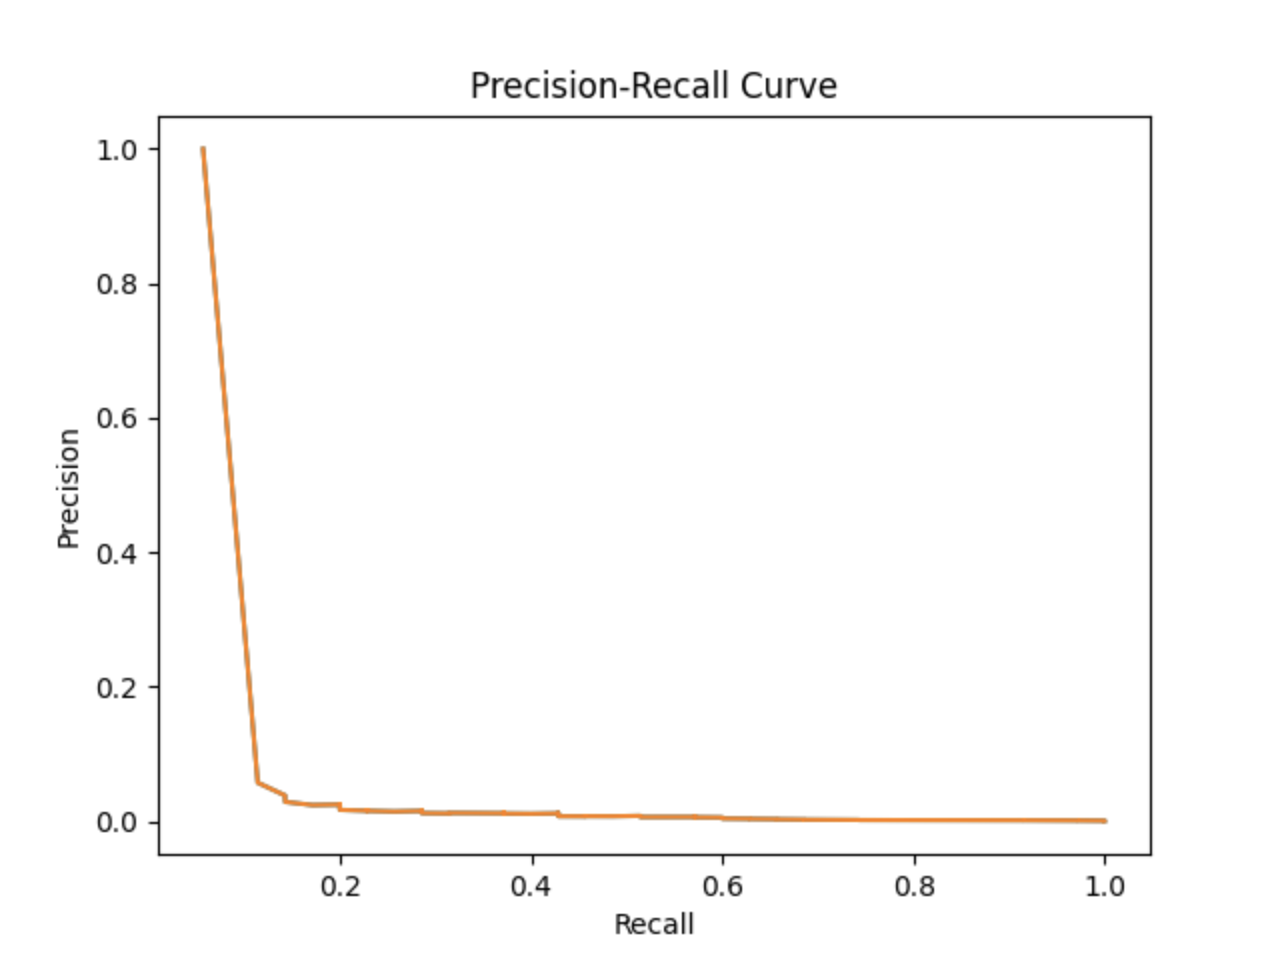
\includegraphics[width=\linewidth]{Precision-Recall.png}
    \caption{Precision-Recall Curve}
    \label{fig:enter-label}
\end{figure}

\end{document}
